\documentclass[tikz,border=8pt]{standalone}

\usepackage[T1]{fontenc}
\usepackage{helvet}
\renewcommand{\familydefault}{\sfdefault}
\usetikzlibrary{arrows.meta,backgrounds,fit,positioning}

\definecolor{ink}{HTML}{253238}
\definecolor{line}{HTML}{526A72}
\definecolor{inputfill}{HTML}{F4E7CF}
\definecolor{processfill}{HTML}{DDEFF2}
\definecolor{rankfill}{HTML}{D9E8E6}
\definecolor{supportfill}{HTML}{ECEFF1}
\definecolor{outputfill}{HTML}{F3DFA2}
\definecolor{guardfill}{HTML}{F3D6C8}
\definecolor{lanefill}{HTML}{F7FAFA}

\begin{document}
\hyphenpenalty=10000
\exhyphenpenalty=10000
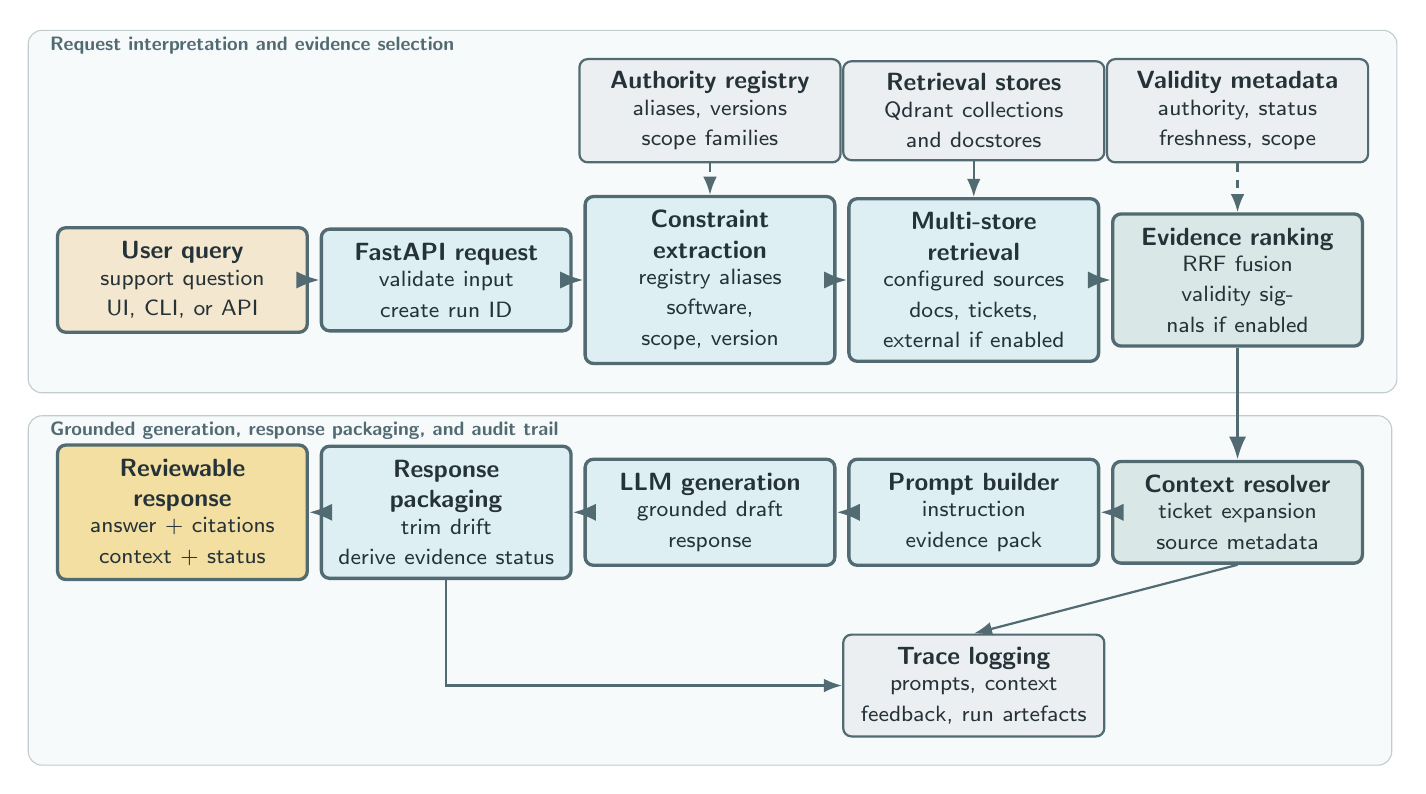
\begin{tikzpicture}[
  font=\small,
  text=ink,
  box/.style={
    draw=line,
    very thick,
    rounded corners=3pt,
    align=center,
    inner sep=5pt,
    minimum height=1.12cm,
    text width=2.82cm
  },
  support/.style={
    draw=line,
    thick,
    rounded corners=3pt,
    align=center,
    inner sep=4.5pt,
    minimum height=0.92cm,
    text width=3.00cm,
    fill=supportfill
  },
  input/.style={box, fill=inputfill},
  process/.style={box, fill=processfill},
  rank/.style={box, fill=rankfill},
  output/.style={box, fill=outputfill},
  guard/.style={box, fill=guardfill},
  arrow/.style={-Latex, very thick, draw=line},
  dataarrow/.style={-Latex, thick, draw=line},
  metaarrow/.style={-Latex, thick, dashed, draw=line},
  note/.style={font=\scriptsize, text=line, align=center},
  lane/.style={
    draw=line!35,
    rounded corners=5pt,
    fill=lanefill,
    inner sep=10pt
  }
]

% Request interpretation and evidence selection
\node[input] (query) at (0,2.4) {\textbf{User query}\\{\footnotesize support question\\UI, CLI, or API}};
\node[process] (api) at (3.35,2.4) {\textbf{FastAPI request}\\{\footnotesize validate input\\create run ID}};
\node[process] (constraints) at (6.70,2.4) {\textbf{Constraint extraction}\\{\footnotesize registry aliases\\software, scope, version}};
\node[process] (retrieve) at (10.05,2.4) {\textbf{Multi-store retrieval}\\{\footnotesize configured sources\\docs, tickets, external if enabled}};
\node[rank] (rerank) at (13.40,2.4) {\textbf{Evidence ranking}\\{\footnotesize RRF fusion\\validity signals if enabled}};

\draw[arrow] (query) -- (api);
\draw[arrow] (api) -- (constraints);
\draw[arrow] (constraints) -- (retrieve);
\draw[arrow] (retrieve) -- (rerank);

% Generation and validation path
\node[rank] (context) at (13.40,-0.55) {\textbf{Context resolver}\\{\footnotesize ticket expansion\\source metadata}};
\node[process] (prompt) at (10.05,-0.55) {\textbf{Prompt builder}\\{\footnotesize instruction\\evidence pack}};
\node[process] (generate) at (6.70,-0.55) {\textbf{LLM generation}\\{\footnotesize grounded draft\\response}};
\node[process] (package) at (3.35,-0.55) {\textbf{Response packaging}\\{\footnotesize trim drift\\derive evidence status}};
\node[output] (answer) at (0,-0.55) {\textbf{Reviewable response}\\{\footnotesize answer + citations\\context + status}};

\draw[arrow] (rerank.south) -- (context.north);
\draw[arrow] (context) -- (prompt);
\draw[arrow] (prompt) -- (generate);
\draw[arrow] (generate) -- (package);
\draw[arrow] (package) -- (answer);

% Side inputs and guard rails
\node[support] (stores) at (10.05,4.55) {\textbf{Retrieval stores}\\{\footnotesize Qdrant collections\\and docstores}};
\node[support] (metadata) at (13.40,4.55) {\textbf{Validity metadata}\\{\footnotesize authority, status\\freshness, scope}};
\node[support] (registry) at (6.70,4.55) {\textbf{Authority registry}\\{\footnotesize aliases, versions\\scope families}};
\node[support] (trace) at (10.05,-2.75) {\textbf{Trace logging}\\{\footnotesize prompts, context\\feedback, run artefacts}};

\draw[dataarrow] (stores.south) -- (retrieve.north);
\draw[metaarrow] (metadata.south) -- (rerank.north);
\draw[metaarrow] (registry.south) -- (constraints.north);
\draw[dataarrow] (context.south) -- (trace.north);
\draw[dataarrow] (package.south) |- (trace.west);

% Lane background
\begin{scope}[on background layer]
  \node[lane, fit=(query)(api)(constraints)(retrieve)(rerank)(stores)(metadata)(registry)] (selectlane) {};
  \node[lane, fit=(context)(prompt)(generate)(package)(answer)(trace)] (genlane) {};
\end{scope}

\node[note, anchor=west] at ([xshift=0.16cm,yshift=-0.20cm]selectlane.north west) {\textbf{Request interpretation and evidence selection}};
\node[note, anchor=west] at ([xshift=0.16cm,yshift=-0.20cm]genlane.north west) {\textbf{Grounded generation, response packaging, and audit trail}};

\end{tikzpicture}
\end{document}
